
\chapter{Allgemeine Untis-Bedienungshinweise}

Guten Tag! Ich habe ein kleines Handbuch erstellt, welches den Ein- bzw. Umstieg zur Untis 2015 erleichtern soll und die Zusammenhänge mit dem THM Organizer Software verdeutlicht.\\
\\
Untis 2015 bietet viele neue Funktionen, welche die Arbeit mit Untis erheblich vereinfachen. Außerdem bietet die Software nun viele Einstellungsmöglichkeiten um die Darstellung bequemer und persönlicher zu gestalten. Das folgende Kapitel wird Ihnen dabei behilflich sein, Untis an Ihre persönlichen Bedürfnisse anzupassen und den Umgang mit der Vielfalt an Ansichten zu erleichtern.\\
\\

\section{Ribbon-Oberfläche und neue Menüführung}

Sehr auffällig bei Untis 2015 ist der Umstieg auf die, für Benutzer von Microsoft-Produkten vertraute, Ribbon-Oberfläche. 

\begin{figure}[h]
	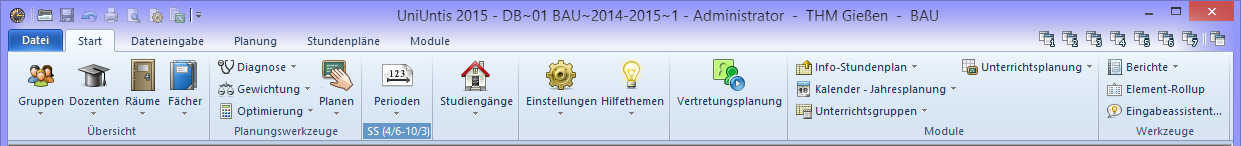
\includegraphics[width=1\textwidth]{ribbon-menu}
	\vspace{-15pt}
	\caption{Ribbon Oberfläche}
	\label{fig:ribbon}
\end{figure}

\noindent
Dies führt zu einem übersichtlicherem Hauptmenü mit wenigen Menüpunkten. Außerdem sind viele der Untermenüpunkte sofort sichtbar, was die Navigation deutlich erleichtert. Auch viele der Ressourcen-bezogenen Menüpunkte wurden unter den entsprechenden Ressourcen zusammengefasst. Beispielsweise sind die Ansichten für Gruppenverwaltung, Unterrichte (Gruppen-bezogen), und sämtliche Gruppenpläne jetzt Untermenüpunkte von Gruppen.  

\subsection{Menü Personalisierung}

Neu ist auch die Möglichkeit, die Menüleiste nach Belieben anzupassen. Unter Anderem die in der Schnellzugriff-Leiste angebotenen Ansichten, die deren Positionierung, und die Anzeige der Ribbon-Oberfläche.\\

\begin{wrapfigure}{r}{0.4\textwidth}
	\vspace{-4pt}
	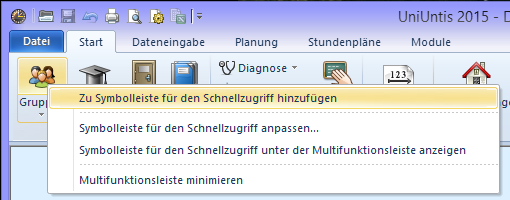
\includegraphics[width=.38\textwidth]{context-menu}
	\vspace{-5pt}
	\caption{Kontext Menü}
	\label{fig:context-menu}
	\vspace{50pt}
	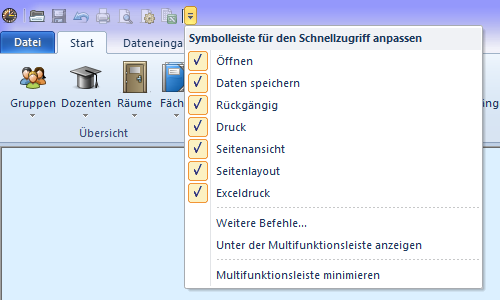
\includegraphics[width=.38\textwidth]{remove-quick-access-item}
	\vspace{-5pt}
	\caption{Vordefinierte Symbole\newline Entfernen}
	\label{fig:remove-quick-access-item}
	\vspace{4pt}
\end{wrapfigure}

\noindent
Um der Schnellzugriff-Leiste eine Ansicht hinzuzufügen, öffnet man das Kontext-Menü (Rechtsklick) und klickt auf den ersten Eintrag 'Zu Symbolleiste für den Schnellzugriff hinzufügen'. Hiermit kann man häufig verwendete Ansichten schneller, bzw. ohne die Menüführung zu verwenden, öffnen.\\
\\
Es gibt zwei Methoden, Elemente aus der Schnellzugriff-Leiste zu entfernen. Wenn das Symbol nicht standardmäßig angeboten wird (falls Sie das Symbol selbst hinzugefügt haben), verwendet man ebenfalls das Kontext Menü zum entfernen der Elemente. Nach einem Rechtsklick auf ein solches Symbol erscheint als erste Option 'Aus Symbolleiste für den Schnellzugriff entfernen', welche das Symbol von der Leiste entfernt.\\
\\
Um vordefinierte Symbole wie 'Öffnen' oder 'Datei Speichern' zu entfernen, klickt man auf das Symbol (kleiner Pfeil nach unten) direkt rechts von der Leiste. Dies öffnet ein neues Kontext-Menü, welches die vordefinierten dargestellten Symbole mit einem Häkchen davor anzeigt. Um die unerwünschten Symbole aus der Liste zu entfernen, muss nun das entsprechende Häkchen entfernt werden.\\
\\
Da die Ribbon-Oberfläche die Arbeitsfläche verringert, bietet die Software über das Kontext-Menü die Möglichkeit, diese zu minimieren. Dies hat als Folge, dass die Ribbon-Oberfläche nur sichtbar wird wenn man einen der Hauptmenüpunkte anklickt. Das Standardverhalten kann man von überall in der Menüleiste, durch das Entfernen der entsprechenden Häkchen vom Kontext-Menü, wiederherstellen.\\
\\
Letztlich kann man auch die Schnellzugriff-Leiste unterhalb der Ribbon-Oberfläche darstellen lassen, in dem man im Kontext-Menü auf den dritten Punkt 'Symbolleiste für den Schnellzugriff unter der Multifunktionsleiste anzeigen' klickt. So eingestellt, kann man die Leiste auf ihre Ursprungsposition bringen, in dem man nochmal auf den dritten Punkt des Kontext-Menüs klickt.

\newpage

\subsection{Standard Fenstergruppen}
\label{sec:standard-fenstergruppen}

\begin{wrapfigure}{r}{0.41\textwidth}
	\vspace{-14pt}
	\centering
	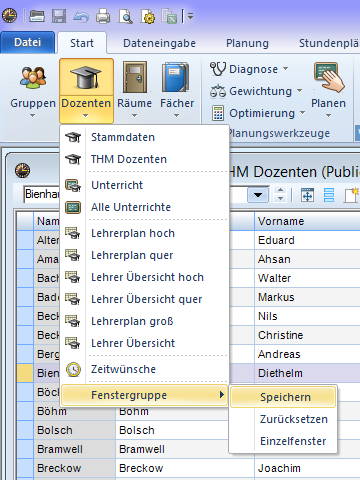
\includegraphics[width=.38\textwidth]{default-window-grouping}
	\vspace{-5pt}
	\caption{Felder der Ansicht Icon}
	\label{fig:default-window-grouping}
\end{wrapfigure}

Eine weitere Neuheit, verbunden mit der Zusammenführung der Ressourcen-Ansichten, sind die Standard-Fenstergruppen. Wenn man auf die großen Symbole der Hauptressourcen klickt, öffnet sich erstmal eine vordefinierte Gruppierung von Ansichten, welche mit dieser Ressource zusammenhängen. Durch einen Klick auf das Tür-Symbol, zum Beispiel, werden alle bereits geöffneten Ansichten geschlossen und die Ansichten Stammdaten, Zeitwünsche, Raumplan Hoch, und Unterricht geöffnet.\\
\\
Obwohl die voreingestellten Ansichten nicht wirklich brauchbar sind, deuten sie an,  wie vielseitig sie verwendbar sind. Um eine Fenstergruppe zu erstellen, öffnen Sie vorerst die Ansichten und Formate, mit welchen Sie gerne arbeiten möchten und verteilen Sie diese so auf der Arbeitsfläche wie sie Ihnen am Besten gefallen.\\
\\
Danach offnen Sie den Menüeintrag \texttt{Fenstergruppe}, unter der Ressource mit dem Sie die Fenster assoziieren möchten, und klicken Sie auf speichern wie in \figref{fig:default-window-grouping} dargestellt. Weitere Informationen zu Fenstergruppen in \secref{sec:fenstergruppen}.

\section{Fensterbereiche}
\label{sec:fensterbereiche}

Jede Untis Fenster hat zwei Bereiche mit Informationsgehalt. Der obere Bereich ist der sogenannte 'Rasteransicht' und ist für die Hauptdarstellung und -bearbeitung der Informationen gedacht. Auch wenn die zu darstellende Informationen und die damit verbundene Bearbeitung zwischen die einzelne Ansichten recht unterschiedlich ist, ist sie immer vorhanden.\\
\\
In Stammdaten- und Unterricht-Ansichten kann man in diesem Bereich Informationen zu den unterschiedlichen Ressourcen eintragen. Welche Daten einzupflegen sind, wird in die \chapref{chap:data}, und \chapref{chap:lessons}, erläutert. In Stundenplan-Ansichten kann man in diesem Bereich die Ressourcenpläne gestalten, sehe \chapref{chap:schedules}.\\
\\
Der untere Bereich ist in der Stammdaten- und Unterricht-Ansichten ein 'Formularansicht'. Dieser Bereich ist per Default versteckt und muss, falls gewollt, mit dem nach-unten-zeigender Pfeilkopf in der untere linke Ecke des Fensters eingeblendet werden. Hier werden alle verfügbare Angaben zur Ressource in einem Formular dargestellt. Um den Benutzer nicht zu überfordern, sind diese in verschiedenen Themenbereiche aufgeteilt. Diese werden wiederum auf eine Reiterleiste abgebildet.\\

\newpage

\noindent
In Stundenplan-Ansichten ist dieser Bereich immer eingeblendet. Wenn man eine geplante oder ungeplante Unterrichtsstunde klickt, wird dessen Informationen in diesem Bereich angezeigt. Sollte man eine ungeplante Stunde über den Stundenplan hin- und herziehen, werden Informationen zu den Unterrichten angezeigt mit dem die zu planende Unterrichtsstunde kollidieren würde.\\

\section{Fensterbedienung}

\begin{wrapfigure}{r}{0.4\textwidth}
	\vspace{-14pt}
	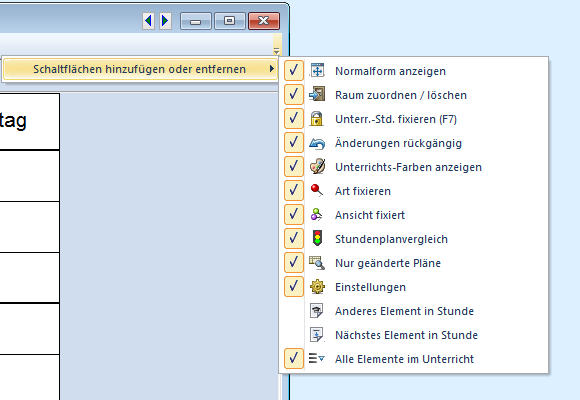
\includegraphics[width=.38\textwidth]{window-personalization}
	\vspace{-5pt}
	\caption{Fenster Personalisierung}
	\label{fig:window-personalization}
\end{wrapfigure}

Ab Untis 2015 sind die Symbolleisten der Fenster nicht mehr frei verschiebbar, dafür kann man sie ähnlich wie die Schnellzugriffs-Leiste, über der Pfeil nach unten an der rechten Seite der jeweilige Symbolleiste ein- oder ausblenden. Ein Klick auf den Pfeil öffnet ein Menü, dessen Länge von der Anzahl der nicht angezeigten Symbole abhängt. Wichtig ist hier der letzte Eintrag, \texttt{Schaltflächen hinzufügen oder entfernen}.\\
\\
Ein Klick auf den Eintrag, 'Schaltflächen hinzufügen oder entfernen' blendet ein weiteres Menü ein, mit welchem man die angezeigten Elemente nach Belieben anpassen kann. Zu berücksichtigen ist hierbei, dass die Elemente, die zur Auswahl stehen, vom jeweiligen Fenstertyp abhängig sind. Stammdaten-Fenstern stehen beispielsweise teilweise andere Bediensymbolen zur Verfügung, als Übersichtsplänen. Es ist sogar so, dass zwischen unterschiedlichen Fenstertypen unterschiedliche Funktionalität hinter den gleichen Symbolen steckt. Mehr Informationen dazu später in dieser und den ansichtsspezifischen Sektionen.\\
\\
Im ersten Teil des Abschnitts wird die überarbeitete Auswahlbox kurz erläutert. Danach werden die mit der Symbolleiste verbundenen Aktionen angesprochen, welche einfache Aktionen durchführen oder weitere Schnittstellen öffnen. Der Einfachheit halber wird die Symbolleiste 'Aktionen' benannt. Im dritten Teil werden Bedienfunktionen, welche erst mit der Eingabe und Anzeige von Daten einleuchten können, beschrieben, im Folgenden als Fenster-Aktionen benannt.

\subsection{Auswahl / Suche}

Die Auswahlbox in Untis Version 2015 wurde deutlich überarbeitet und bietet viele neue Verbesserungen. Die statische Auswahl wächst nun dynamisch in die Breite. Damit werden die, für gewöhnlich aussagekräftigeren, Langnamen immer angezeigt.\\

\begin{wrapfigure}{r}{.4\textwidth}
	\vspace{-19pt}
	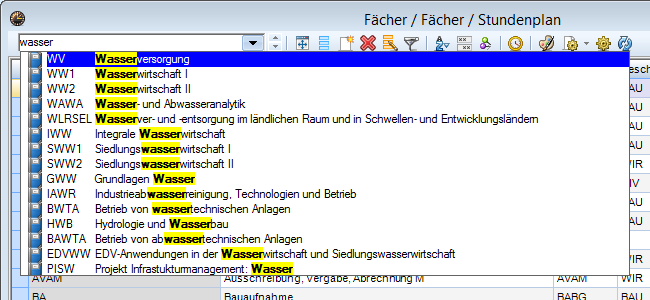
\includegraphics[width=.38\textwidth]{search-field}
	\vspace{-5pt}
	\caption{Suchen}
	\label{fig:search-field}
	\vspace{-15pt}
\end{wrapfigure}

\noindent
Die Auswahlbox als solche ist jedoch nebensächlich geworden, da beim Eintippen die kompletten Inhalte der Kurz- und Langnamen durchsucht werden. Bei der Eingabe eines einzelnen Zeichens grenzt Untis die Ergebnisse bereits ein und zeigt diese auch sofort in einer Drop-Down Liste an. Bei vielen Ressourcen ist es daher immer schneller,  die Auswahlbox als Suchfeld zu verwenden. 

\subsection{Symbolleiste Aktionen}
\label{sec:symbolleiste-aktionen}

Im Folgenden werden die typischen Symbole der Stammdaten-, Unterrichts- und Stundenplansansichten kurz erläutert. Für uns überflüssige Symbole werden nicht angesprochen.\\

\subsubsection{Alle Elemente im Unterricht}
{\small\textit{verfügbar in Einzelplan Ansichten\\}\par}

\begin{wrapfigure}{r}{.06\textwidth}
	\vspace{-50pt}
	
\includegraphics[width=.06\textwidth]{alle-elemente-im-unterricht-symbol}
	\vspace{-35pt}
\end{wrapfigure}

\noindent
Dieses Symbol erzeugt eine kleine Reiterleiste im oberen linken Eck eines Einzelplans. Falls man eine Unterrichtsstunde im Plan auswählt, werden Reiter erstellt und dieser Reiterleiste hinzugefügt. Man kann auf die Elemente dieser Leiste klicken, um die Einzelpläne der verbundenen Ressourcen schnell anzuschauen. Standardmäßig eingeschaltet, lässt das Ausschalten einen Reiter verschwinden und man bekommt, sollte man einen anderen Plan angeschaut haben, den Ursprungsplan dargestellt.\\

\subsubsection{Änderungen Rückgängig}
{\small\textit{explizit verfügbar in allen Stundenplan-Ansichten\\}\par}

\begin{wrapfigure}{r}{.05\textwidth}
	\vspace{-50pt}
	
\includegraphics[width=.05\textwidth]{anderungen-ruckgangig-symbol}
	\vspace{-35pt}
\end{wrapfigure}

\noindent
Änderungen werden in Untis protokolliert und können rückgängig gemacht werden. Stundenplänen steht dieses Symbol in der Symbolleiste zur Verfügung. Ein Rückgängig-Befehl kann jedoch in jeder Ansicht verwendet werden. In den Ansichten, in welchen das Symbol nicht angezeigt wird, kann man auf die Tastenkombination STRG + Z zurückgreifen oder das Symbol in der Schnellzugriff-Leiste betätigen.\\
\\
\textbf{Vorsicht}: \textit{Diese Funktion protokolliert im aktuellen Stand die zugewiesenen Räume in der Planung nicht mit! Manuell zugewiesene Räume gehen verloren!}\\

\subsubsection{Ansicht Fixiert}
{\small\textit{verfügbar in allen Fenster Ansichten\\}\par}

\begin{wrapfigure}{r}{.05\textwidth}
	\vspace{-50pt}
	
\includegraphics[width=.05\textwidth]{ansicht-fixiert-symbol}
	\vspace{-35pt}
\end{wrapfigure}

\noindent
Diese Aktion beeinflusst das Verhalten des Fensters in Abhängigkeit zu den ausgewählten Elementen anderer Fenster. Standardmäßig ist diese ausgestellt, d.h. das Fenster wird von Benutzerinteraktion mit anderen Fenstern beeinflusst. Dies kann oft von Vorteil sein, z.B. wenn man Ressourcenpläne von unterschiedlichen Typen gleichzeitig untersucht. Sobald man die Pläne zweier Ressourcen des gleiche Ressourcentyps untersucht, ist es ratsam einen dieser Pläne zu fixieren, da sich die ausgewählte Ressourcen sonst den Plänen anpassen.\\

\newpage

\subsubsection{Einstellungen}
\label{sec:einstellungen}
{\small\textit{verfügbar in allen Fenster Ansichten\\}\par}

\begin{wrapfigure}{r}{.05\textwidth}
	\vspace{-50pt}
	
\includegraphics[width=.05\textwidth]{einstellungen-symbol}
	\vspace{-35pt}
\end{wrapfigure}

\noindent
Obwohl in allen Fenster-Ansichten verfügbar, verbirgt sich hinter dem Einstellungs-Symbol für jede Ansicht eine abweichende Funktionalität.\\
\\
Bei Stammdaten- und Unterricht-Ansichten sind die Einstellungen hauptsächlich auf die Auswahl der Schriftart, -größe und - stil begrenzt. Bei Unterrichts-Ansichten kann man zusätzlich entscheiden, ob die Summen-Zeile und geerbte Kennzeichen angezeigt werden sollen. Die Option ``nur eine Woche" \hspace{1pt} scheint die Anzeige der Unterrichtstunden auf die Stunden, die in der erste Schulwoche stattfinden, einzugrenzen. Eine Möglichkeit, weitere Wochen anzusehen, scheint nicht verfügbar zu sein. Diese Option sollte Ihrerseits nicht gesetzt werden.\\
\\
Bei Stundenplan-Ansichten öffnen sich weitere Einstellungen, welche später in \secref{sec:druck-einstellungen}, und \secref{sec:stundenplan-einstellungen}, näher erläutert werden.

\subsubsection{Elementart}
{\small\textit{verfügbar in Stundenplan-Ansichten\\}\par}

\noindent %this
Erlaubt einen direkt von einer Ressourcenart zur anderen zu wechseln. Das Icon ist abhängig vom ausgewählten Ressourcentyp. Obwohl Studenten als Ressourcentyp zur Auswahl steht, scheint dieser nicht implementiert zu sein. Bitte daher nicht benutzen.

\subsubsection{Erweitertes Entkoppeln}
{\small\textit{verfügbar in Unterricht-Ansichten\\}\par}

\begin{wrapfigure}{r}{.05\textwidth}
	\vspace{-50pt}
	
\includegraphics[width=.05\textwidth]{erweitertes-entkoppeln-symbol}
	\vspace{-35pt}
\end{wrapfigure}

\noindent
Dieses Symbol öffnet die Entkoppeln-Ansicht, zur Umgestaltung von ausgewählten Unterrichtskopplungszeilen zu eigenständigen Unterrichten. Mehr dazu in \secref{sec:kopplungszeilen}.

\subsubsection{Farbe des Elements}
{\small\textit{verfügbar in Stammdaten- und Unterricht-Ansichten\\}\par}

\begin{wrapfigure}{r}{.05\textwidth}
	\vspace{-50pt}
	
\includegraphics[width=.05\textwidth]{farbe-des-elements-symbol}
	\vspace{-35pt}
\end{wrapfigure}

\noindent
Dieses Symbol öffnet die Farb-Ansicht. Hier kann man die Vordergrund- (Schrift) sowie Hintergrund-Farben von Elementen einstellen. Untis hat von Haus aus eine Palette mit 48 Farben und lässt bis zu 12 eigene Definitionen zu. Man kann die Farb-Einstellungen eines Elements einfach entfernen, indem man ein Häkchen bei 'keine Farben' setzt. Sofern man die Ansicht noch nicht geschlossen hat, kann man die bisherigen Einstellungen durch das Entfernen des Häkchens wiederherstellen. Des Weiteren kann man Stammdaten-Elemente so einrichten, dass neu angelegte Elemente automatisch Farben zugewiesen bekommen.\\

\newpage

\subsubsection{Felder der Ansicht}
\label{sec:felder-der-ansicht}
{\small\textit{verfügbar in Stammdaten- und Unterricht-Ansichten\\}\par}

\begin{wrapfigure}{r}{.05\textwidth}
	\vspace{-50pt}
	
\includegraphics[width=.05\textwidth]{felder-der-ansicht-symbol}
	\vspace{-35pt}
\end{wrapfigure}

\noindent
Untis verlangt von Haus aus nur das Nötigste an Informationen, um Daten anzulegen. Bei Stammdaten wird nur der \texttt{Name} (Kurzname) der Ressource und bei Unterrichten nur eine Anzahl der zu haltende Stunden benötigt. Jedoch hat jeder Ressourcentyp einen Standardsatz an Zusatzfeldern, welche standardmäßig eingeblendet sind. Diese sind für unsere Zwecke jedoch nicht ausreichend und ansatzweise auch nicht passend.\\

\begin{wrapfigure}{r}{0.4\textwidth}
	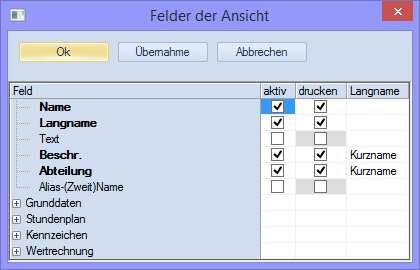
\includegraphics[width=.38\textwidth,right]{felder-der-ansicht}
	\vspace{-15pt}
	\caption{Felder der Ansicht}
	\label{fig:felder-der-ansicht}
	\vspace{10pt}
\end{wrapfigure}

\noindent
Damit wir möglichst aussagekräftige Daten im System haben, müssen die Felder erst angepasst werden. Diese werden über das Symbol, bzw. der Ansicht \texttt{Felder der Ansicht} eingeblendet. Hier kann man überflüssige Angaben, wie \texttt{Hohlstunden}, ausblendet und wichtige wie \texttt{Schulübergreifender Name} eingeblendet werden. Die spezifische Felder werden bei der jeweilige Ansicht näher erläutert.\\
\\
Sofern die Angabe eine weitere verwaltete Ressource ist, kann man auswählen, wie die Angabe dieser Ressource erfolgen soll. Möglich sind der \texttt{Kurzname}, der \texttt{Langname} (bzw. \texttt{Nachname}) oder beide Namen mit einem Schrägstrich ``/" getrennt.\\

\subsubsection{Felder mit Inhalt}
{\small\textit{verfügbar in Stammdaten- und Unterricht-Ansichten\\}\par}

\begin{wrapfigure}{r}{.05\textwidth}
	\vspace{-50pt}
	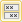
\includegraphics[width=.05\textwidth]{felder-mit-inhalt-symbol}
	\vspace{-35pt}
\end{wrapfigure}

\noindent
Felder mit Inhalt blendet \textbf{alle} mit einem Wert belegten Felder ein. Dies kann hilfreich sein, um sich daran zu erinnern welche Felder mit Werten zu belegen sind. Es kann auch ein etwas tieferes Verständnis der Abläufe in Untis verschaffen, da neben den vom Benutzer eingegebenen Werte auch die dynamisch vom Programm berechneten werte angezeigt werden.\\

\subsubsection{Fenster Aktualisieren}
{\small\textit{verfügbar in Stammdaten- und Unterricht-Ansichten\\}\par}

\begin{wrapfigure}{r}{.05\textwidth}
	\vspace{-50pt}
	
\includegraphics[width=.05\textwidth]{fenster-aktualisieren-symbol}
	\vspace{-35pt}
\end{wrapfigure}

\noindent
Dieses Symbol aktualisiert das Fenster. Untis sucht nach lokalen und externen Änderungen und pflegt gefundene Datensätze sortiert ein.\\

\newpage

\subsubsection{Klassenzeitraster}
{\small\textit{verfügbar in Gruppen-Stammdaten Ansichten\\}\par}

\begin{wrapfigure}{r}{.05\textwidth}
	\vspace{-50pt}
	
\includegraphics[width=.05\textwidth]{klassenzeitraster-symbol}
	\vspace{-35pt}
\end{wrapfigure}

\noindent
Hier wird ein Fenster geöffnet, in dem man den Tagesablauf einer Gruppe anhand der assoziierten Raster für die automatische/optimierte Planung festlegen kann. Da dieses nicht vollständig implementiert zu sein scheint, sollten Sie es nicht benutzen.\\

\subsubsection{Koppeln}
{\small\textit{verfügbar in Unterricht-Ansichten\\}\par}

\begin{wrapfigure}{r}{.05\textwidth}
	\vspace{-50pt}
	
\includegraphics[width=.05\textwidth]{koppeln-symbol}
	\vspace{-35pt}
\end{wrapfigure}

\noindent
Dieser Symbol öffnet eine Ansicht, in welcher mehrere getrennte Unterrichte zu einem Unterricht mit mehreren Kopplungszeilen zusammenfügt werden kann. Nähere Informationen dazu in \secref{sec:kopplungszeilen}.\\

\subsubsection{Lehrer-Vorschlag}
{\small\textit{verfügbar in Unterricht-Ansichten\\}\par}

\begin{wrapfigure}{r}{.06\textwidth}
	\vspace{-50pt}
	
\includegraphics[width=.06\textwidth]{lehrer-vorschlag-symbol}
	\vspace{-35pt}
\end{wrapfigure}

\noindent
Der Lehrer-Vorschlag bietet Ihnen ein kleines Menü, in welchem die Möglichkeiten der Lehrer-Vorschlags-Ansicht (das Leeren des Dozent-Feldes, Verwendung des Vorjahres-Lehrer) aufgelistet sind.\\
\\
Die Lehrer-Vorschlag-Ansicht listet alle Dozenten anhand ihrer von Untis eingetragenen/kalkulierten Ist, Soll und Ist-Soll Werte auf. Diese kann von Nutzen sein, wenn man nach einem Dozenten mit freien Kapazitäten sucht. Standardmäßig werden die Dozenten nach ihren noch zu führenden Stunden aufgelistet, jedoch können diese Angaben nach allen Spalten sortiert werden.\\
\\
Die Option Vorjahres-Lehrer bezieht sich auf Klassen-Lehrer, wie man sie von der Grundschule oder dem Gymnasium kennt und ist für unsere Zwecke nicht zu gebrauchen.

\subsubsection{Löschen}
{\small\textit{verfügbar in Stammdaten- und Unterricht-Ansichten\\}\par}

\begin{wrapfigure}{r}{.05\textwidth}
	\vspace{-50pt}
	
\includegraphics[width=.05\textwidth]{loschen-symbol}
	\vspace{-35pt}
\end{wrapfigure}

\noindent %this
Entfernt alle markierte Einträge, ggf. nur in der aktuelle Periode. Die Einträge können, unter Umständen, weiterhin in andere Perioden bestehen.

\subsubsection{Normalform Anzeigen}
{\small\textit{verfügbar in allen Fenster Ansichten\\}\par}

\begin{wrapfigure}{r}{.05\textwidth}
	\vspace{-50pt}
	
\includegraphics[width=.05\textwidth]{normal-form-anzeigen-symbol}
	\vspace{-35pt}
\end{wrapfigure}

\noindent
Die Schaltfläche \texttt{Normalform Anzeigen} bewirkt, dass die Größe des Fensters sich der Höhe und Breite der angezeigten Zeilen und Spalten anpasst. Bei einer geringen Anzahl an Einträgen wird die Höhe des Fensters ggf. schrumpfen. Wohingegen bei vielen Zeilen, kann die komplette Höhe der Arbeitsfläche eingenommen werden.\\
\\
Zusätzlich führt das Klicken auf dieses Symbol bei manchen Ansichten eine Art Zurücksetzen durch. Bei Gruppenstundenplänen zum Beispiel wird man zurück zum Gruppenplan vom letzten angeklickten Unterricht geführt. Dies kann eine ganz andere Gruppe sein als jene, mit der man angefangen hat.

\subsubsection{Nur geänderte Pläne}
{\small\textit{verfügbar in Stundenplan-Ansichten\\}\par}

\begin{wrapfigure}{r}{.05\textwidth}
	\vspace{-50pt}
	
\includegraphics[width=.05\textwidth]{nur-geanderte-plane-symbol}
	\vspace{-35pt}
\end{wrapfigure}

\noindent
Diese Funktion soll der Vergleich zwischen zweier Pläne auf das Geänderte einschränken. Da die Vergleichsfunktion nicht funktioniert, könnte ich das nicht ausprobieren.

\subsubsection{Raum Zuordnen / Löschen}
\label{subsubsec:raum-zuordnen-loschen}
{\small\textit{verfügbar in Unterricht-Ansichten\\}\par}

\begin{wrapfigure}{r}{.05\textwidth}
	\vspace{-50pt}
	
\includegraphics[width=.05\textwidth]{raum-zuordnen-loschen-symbol}
	\vspace{-35pt}
\end{wrapfigure}

\noindent
Dieses Symbol, oder der entsprechende Unterrichtsstunden-Kontextmenüeintrag, öffnet die Ansicht \texttt{Raum zuordnen / löschen} für die im Stundenplan selektierte Stunde. Hier kann man alle Räume einer Periode, mit ausgewählten Informationen wie \texttt{Besetzt} (ob der Raum schon in der Stunde verplant ist), \texttt{Kapazität} (Anzahl der Sitzplätze), ob ein Raum als \texttt{Ausweichraum} für den gewünschten Raum eingetragen ist, sowie die Raumgruppenzugehörigkeit, sehen.\\

\begin{wrapfigure}{r}{0.3\textwidth}
	\vspace{-14pt}
	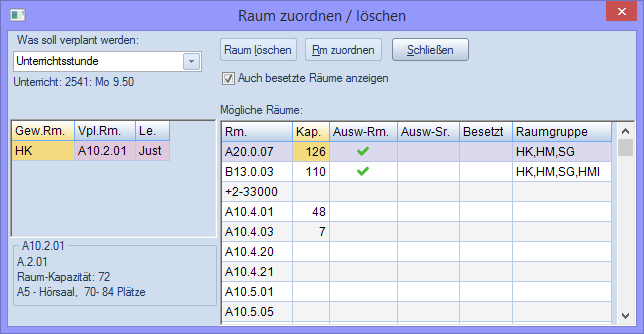
\includegraphics[width=.29\textwidth,right]{raum-zuordnen-loschen}
	\vspace{-15pt}
	\caption{Raum zuordnen / löschen}
	\label{fig:raum-zuordnen-loschen}
\end{wrapfigure}

\noindent
Man kann Räume zuordnen, indem man einen Raum selektiert und den Knopf \texttt{Rm zuordnen} drückt, oder zweimal auf den gewünschten Raum klickt. Man kann auf ähnliche Weise die Zuordnung löschen, indem man \texttt{Raum löschen} drückt oder zweimal auf den nicht erwünschten Raum klickt.\\
\\
Besetzte Räume werden mit einem Häkchen in der entsprechenden Spalte dargestellt. Sobald diese Ansicht geöffnet wird, werden solche Räume entweder unten an der Liste der Räume angehängt oder sogar ausgeblendet. Falls zweites eintreffen sollte, muss man ein Häkchen bei \texttt{Auch besetzte Räume Anzeigen} um diese einzublenden. Auch wenn Räume besetzt sind, kann man dennoch Unterrichtsstunden, wie oben beschrieben, zuweisen. Diese Zuordnung führt zu einer weiteren Warnungs- /Bestätigungsansicht \texttt{Raum nicht frei}.\\

\newpage

\begin{wrapfigure}{r}{0.3\textwidth}
	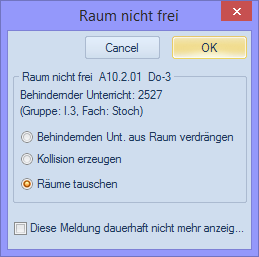
\includegraphics[width=.29\textwidth,right]{raum-nicht-frei}
	\vspace{-15pt}
	\caption{Raum nicht frei}
	\label{fig:raum-nicht-frei}
	\vspace{10pt}
\end{wrapfigure}

\noindent
\texttt{Raum nicht frei} gibt eine kurze Auflistung der Unterrichte, die durch diese Raumbelegung betroffen wären sowie drei Optionen, wie dieser Konflikt gelöst werden könnte: \texttt{Behinderten Unt. aus Raum verdrängen} (andere Unterrichte verlieren ihre Raumzuordnung), \texttt{Kollision erzeugen} (alle Unterrichte behalten ihre Zuordnung und der neue kommt dazu) und \texttt{Räume tauschen} (andere Unterrichte bekommen die vorherige des aktuellen Unterrichts). Alle drei Optionen können zum Einsatz kommen: normalerweise ist \texttt{Kollsion erzeugen} ein sichere Wahl, vorausgesetzt man geht bewusst mit der Erzeugung von Kollisionen um. Unten gibt es eine weitere Einstellungsmöglichkeit, \texttt{Diese Meldung dauerhaft nicht mehr anzeig...}, das setzten dieses Häkchen bewirkt, dass die ausgewählte Option immer verwendet wird und der \texttt{Raum nicht frei}-Ansicht nicht mehr zum Vorschein kommt. Bisher habe ich keine Möglichkeit gefunden, diesen wieder anzeigen zu lassen. \textbf{Sie sollten dieses Häkchen nie setzen.}\\

\subsubsection{Schuljahreskalendar}
{\small\textit{verfügbar in Stammdaten (ausser Fächer) und Unterricht-Ansichten\\}\par}

\begin{wrapfigure}{r}{.05\textwidth}
	\vspace{-50pt}
	
\includegraphics[width=.05\textwidth]{schuljahreskalendar-symbol}
	\vspace{-35pt}
\end{wrapfigure}

\noindent
Bei Stammdaten öffnet dieses Symbol die \texttt{Absenzen}-Ansicht, in welcher man die nicht verfügbaren Tage einer Ressource eintragen kann. Leider scheint diese Funktion nicht vollständig implementiert zu sein und ist an mehreren Stellen fehlerhaft, weshalb sie nicht benutzt werden sollte.\\
\\
Bei Unterrichten wird tatsächlich der Schuljahreskalender geöffnet. Hier wird der Ablauf des Unterrichts, abhängig vom Unterrichtsgruppe (Von- und Bis- Datum), angezeigt. Der Verlauf lässt sich jedoch nicht von dieser Ansicht beeinflussen.\\

\subsubsection{Seitenlayout}
{\small\textit{verfügbar in Stammdaten- und Unterricht-Ansichten\\}\par}

\begin{wrapfigure}{r}{.06\textwidth}
	\vspace{-50pt}
	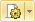
\includegraphics[width=.06\textwidth]{seitenlayout-symbol}
	\vspace{-35pt}
\end{wrapfigure}

\noindent
Ein Klick auf dieses Symbol öffnet ein kleines Menü mit dem Punkten \texttt{Seitenansicht} und \texttt{Seitenlayout}. \texttt{Seitenansicht} beschreibt die druckbare Ausgabe der in dem Fenster erhaltenen Informationen, wohingegen \texttt{Seitenlayout} dessen Gestaltungseinstellungen beinhaltet. Mehr Informationen dazu finden Sie in \secref{sec:druck-einstellungen}.

\subsubsection{Sortieren (automatische)}
{\small\textit{verfügbar in Stammdaten- und Unterricht-Ansichten\\}\par}

\begin{wrapfigure}{r}{.05\textwidth}
	\vspace{-50pt}
	
\includegraphics[width=.05\textwidth]{sortieren-symbol}
	\vspace{-35pt}
\end{wrapfigure}

\noindent
Das Sortieren-Symbol öffnet eine weitere Ansicht, welche das automatische Sortieren ermöglicht. Hier können mehrere Spalten ausgewählt werden, welche als Sortier-Kriterien dienen können. Außerdem kann die Sortierrichtung der Kriterien bestimmt werden.\\

\begin{wrapfigure}{r}{0.35\textwidth}
	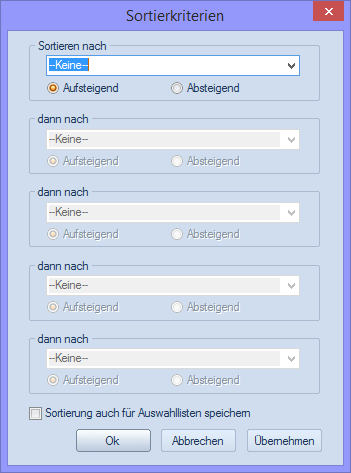
\includegraphics[width=.34\textwidth,right]{sortierkriterien}
	\vspace{-15pt}
	\caption{Sortierkriterien}
	\label{fig:sortierkriterien}
\end{wrapfigure}

\noindent
Das eingestellte Sortierverhalten kann mit \texttt{Ok} oder \texttt{Übernahme} bestätigt werden. Obwohl das Verhalten \textit{permanent} gespeichert wird, kann es nach dem Schließen des Fensters nicht nochmal eingesehen werden. Sollte die Sortierkriterien-Ansicht nach dem Schließen neu aufgerufen werden, werden keine der bereits gespeicherten Einstellungen angezeigt und sie gehen, sollte man sie nicht neu einstellen, nach dem Schließen der Ansicht verloren.\\
\\
Für Ansichten, die mit Stammdaten assoziiert sind, kann man unten in der Ansicht ein Häkchen setzen, welches bewirkt, dass die gespeicherte Sortierung auch für Auswahlboxen für den Ressourcentyp eingehalten wird. Egal in welchem Zustand sich das Sortieren befindet, müssen neue Elemente manuell-automatisch eingerichtet werden. Das bedeutet, dass die Sortierung neu mit Häkchen eingestellt werden muss, damit die gewünschte Sortierung neue Elemente in den Auswahlboxen berücksichtigt.\\

\subsubsection{Stundenplanvergleich}
{\small\textit{verfügbar in Stundenplan-Ansichten\\}\par}

\begin{wrapfigure}{r}{.05\textwidth}
	\vspace{-50pt}
	
\includegraphics[width=.05\textwidth]{stundenplan-vergleich-symbol}
	\vspace{-35pt}
\end{wrapfigure}

\noindent
Dieses Symbol soll es ermöglichen, zwei Stundenpläne zu vergleichen. Laut dem Tooltip soll Untis deswegen ein zweites mal gestartet werden. Diese Funktion führt zum Absturz des Programms daher bitte nicht verwenden.\\

\subsubsection{Unterrichtsstunde Fixieren}
{\small\textit{verfügbar in Stundenplan-Ansichten\\}\par}

\begin{wrapfigure}{r}{.05\textwidth}
	\vspace{-50pt}
	
\includegraphics[width=.05\textwidth]{unterrichtsstunde-fixieren-symbol}
	\vspace{-35pt}
\end{wrapfigure}

\noindent
Sollte man die automatische/optimierte Planung verwenden, verhindert das Betätigen dieses Symbols, dass der geplante Unterricht von diesen Planungsvorgängen geändert wird.\\

\subsubsection{Unterrichtsvergleich}
{\small\textit{verfügbar in Unterricht-Ansichten\\}\par}

\begin{wrapfigure}{r}{.05\textwidth}
	\vspace{-50pt}
	
\includegraphics[width=.05\textwidth]{unterrichtsvergleich-symbol}
	\vspace{-35pt}
\end{wrapfigure}

\noindent
Durch dieses Symbol lassen sich Unterrichte mit dem selben ID aus zwei unterschiedlichen Perioden vergleichen. Einmal angeklickt, öffnet sich eine Ansicht, in welcher man die Periode, sowie die Darstellung der Ergebnisse auswählen kann. Da wir mit großen Änderungen in der Zahl der Studenten, angebotenen Fächer, Studentengruppen und eingesetzten Dozierenden umgehen müssen, bringt uns diese Funktion nicht viel.\\

\subsubsection{Zeitwünsche}
{\small\textit{verfügbar in Stammdaten- und Unterricht-Ansichten\\}\par}

\begin{wrapfigure}{r}{.05\textwidth}
	\vspace{-50pt}
	
\includegraphics[width=.05\textwidth]{zeitwunsche-symbol}
	\vspace{-35pt}
\end{wrapfigure}

\noindent
Zeitwünsche öffnet ein weiteres Fenster, in welchem man Präferenzen zu den Zeiten, in denen Stammdaten zur Verfügung stehen oder Unterrichte gehalten werden sollen, angeben kann. Diese Präferenzen sind abgebildet auf numerische Werte zwischen -3 und +3 mit einem 'X' anstelle eines 0 Wertes. Im Wesentlichen dienen diese Angaben der automatischen/optimierten Stundenplanerstellung. Doch die Angabe -3 hat einen besonderen Stellenwert, da er als absolute Sperre gilt. Sobald die Zeit mit dem Wert -3 belegt ist, wird Untis, sobald man manuell versucht einen Unterricht zu einer gesperrten Zeit zu planen, einen Fehler melden.\\

\begin{wrapfigure}{r}{0.3\textwidth}
	\vspace{-14pt}
	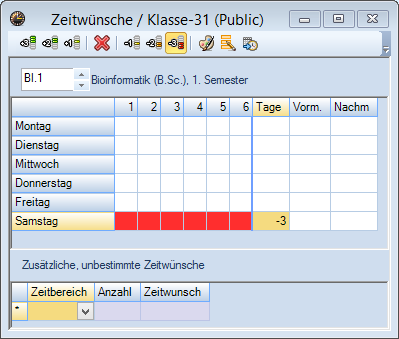
\includegraphics[width=.29\textwidth,right]{zeitwunsche-gruppen}
	\vspace{-15pt}
	\caption{Zeitwünsche Gruppen}
	\label{fig:zeitwunsche-gruppen}
\end{wrapfigure}

\noindent
Die Zeitwünsche-Ansichten haben ein paar wesentliche funktionale Unterschiede in Abhängigkeit zur aufrufenden Ansicht, ggf. dessen Ressourcentyp und der Verwendung der sogenannten Multi-Zeitraster. In \figref{fig:zeitwunsche-gruppen} sehen wir die Zeitwünsche- Ansicht für die Ressource Gruppen. Im Hauptteil des Fensters steht mittig das Zeitraster des Elements. Hier kann man die Werte blockweise eintragen, in denen Unterrichte für diese Ressource stattfinden, bzw. nicht-stattfinden sollen. Bei Gruppen- und Dozenten-Zeitwünschen hat man Zugriff auf erweiterte Hilfsmittel zum Setzen von Werten für ganze Zeitbereiche (Ganztags, Vormittags oder Nachmittags). Räume- und Fächer-Zeitwünsche haben kein solches Hilfsmittel.\\
\\
Da Gruppen immer an ein festes Zeitraster gebunden sind, wird dieses immer in der entsprechenden Zeitwünsche-Ansicht angezeigt. Bei Dozenten, Räumen und Fächern hingegen kann kein eindeutiges Zeitraster angegeben werden. Sollten mehrere Raster vorliegen, sehen ihre Zeitwünsche komplizierter aus, wie in \figref{fig:zeitwunsche-multiraster} veranschaulicht. Hier muss man entsprechende Zeitbereiche mit dem jeweiligen Wert belegen. Die aktuelle Position des Cursors (in Minuten) wird in der ersten Reihe/Spalte angezeigt.

\begin{figure}[h]
	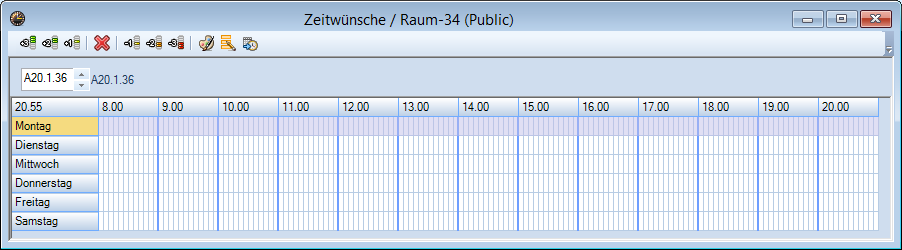
\includegraphics[width=1\textwidth]{zeitwunsche-multiraster}
	\vspace{-15pt}
	\caption{Zeitwünsche Multi-Zeitraster}
	\label{fig:zeitwunsche-multiraster}
\end{figure}

\begin{wrapfigure}{r}{0.3\textwidth}
	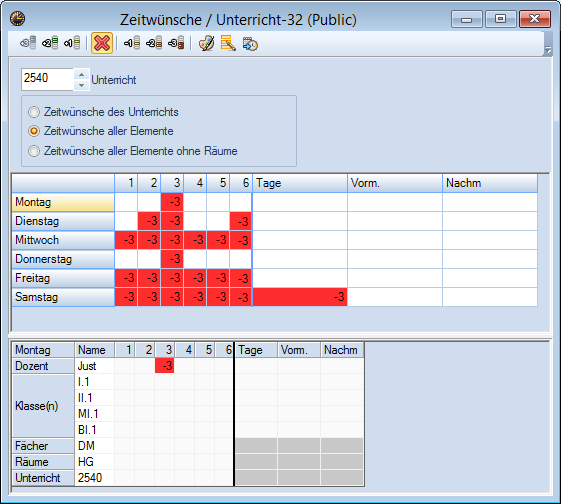
\includegraphics[width=.29\textwidth,right]{zeitwunsche-unterricht}
	\vspace{-15pt}
	\caption{Zeitwünsche Unterrichte}
	\label{fig:zeitwunsche-unterricht}
\end{wrapfigure}

\newpage

\noindent
Unterrichte sind über die zugewiesenen Klassen auch an ein festes Raster gebunden und wie Gruppen und Dozenten kann man auch ganze Zeitbereiche mit einem Wert belegen. Man hat hier die Wahl zwischen drei verschiedenen Darstellungsmöglichkeiten: Unterricht, alle Elemente und alle Elemente ohne Räume. Bei allen drei Möglichkeiten werden automatisch die Zeitwunsch-Werte der assoziierten Ressourcen tageweise unten dargestellt. In \figref{fig:zeitwunsche-unterricht} z.B. sieht man in der Liste der Ressourcen unten eine Sperre bei Frau Just Montags im 3. Block. Bei \texttt{alle Elemente} und \texttt{alle Elemente ohne Räume} werden die Zeitwünsche der assoziierten Ressourcen direkt als die des Unterrichts angezeigt. 

\subsection{Fenster-Aktionen}

\subsubsection{Filter}%everything from here on
{\small\textit{verfügbar in Stammdaten- und Unterricht-Ansichten\\}\par}

\begin{wrapfigure}{r}{.05\textwidth}
	\vspace{-50pt}
	
\includegraphics[width=.05\textwidth]{filter-symbol}
	\vspace{-35pt}
\end{wrapfigure}

\noindent
Filtern ermöglicht das Einschränken der angezeigten Einträge nach der eingetragenen Werte einer Spalte. Man klickt auf das Filter-Symbol um das Filtern zu aktivieren. Danach erscheint eine neue Zeile als erster Eintrag in der Tabelle. Hier trägt man in der Spalte, in der gesucht werden soll, einen Wert ein. Prinzipiell gilt der ganze Wert, es kann aber nach der Anfang des Werts gesucht werden. Zum Beispiel, sollte man im Langname-Spalte der Filterzeile von Raumstammdaten 'A20.*' wäre die Liste auf alle Räume in Gebäude A20.

\subsubsection{Neu}
{\small\textit{verfügbar in Stammdaten- und Unterricht-Ansichten\\}\par}

\begin{wrapfigure}{r}{.05\textwidth}
	\vspace{-50pt}
	
\includegraphics[width=.05\textwidth]{neu-symbol}
	\vspace{-35pt}
\end{wrapfigure}

\noindent
Das Klicken des Neu-Symbols bringt den Fokus zur ersten Spalte der letzten Zeile des Fensters. Man kann auch selber dahin scrollen. Welche Daten einzupflegen sind, wird in die \chapref{chap:data} und \chapref{chap:lessons} näher erläutert.\\

\subsubsection{Serien-Änderung} 
{\small\textit{verfügbar in Stammdaten- und Unterricht-Ansichten\\}\par}

\begin{wrapfigure}{r}{.05\textwidth}
	\vspace{-50pt}
	
\includegraphics[width=.05\textwidth]{serien-anderung-symbol}
	\vspace{-35pt}
\end{wrapfigure}

\noindent
Serienänderungen sind Änderungen, die auf einem bestimmten Bereich oder Einzeleinträge einer Spalte ausgeführt werden. Diese Funktionalität kann bei der Pflege von neuen Informationen, oder dem Löschen von nicht verwendete/gewollte Attribute sehr hilfreich sein. Man kann diese Funktionalität mit oder ohne die vorgesehene Schnittstelle ausführen. Beide Möglichkeiten haben ihre Stärken und setzen Interaktion mit dem Listenbereich des Fensters voraus, denn die zu ändernde Einträge müssen erst ausgewählt werden.\\
\\
Einzeleinträge werden durch mehrfaches \texttt{STRG-Klick} ausgewählt. Bereiche können mit dem Überstreichen mit der Maus markiert werden. Alternativ kann man einen ersten Eintrag auswählen und den letzten des Bereichs mit einem \texttt{Umschalt-Klick} auswählen. Diese Methode, einen Bereich zu markieren, ist nachträglich noch kombinierbar mit der Methode, Eineinträge zu markieren, jedoch nicht in umgekehrt.\\

\begin{figure}[h]
	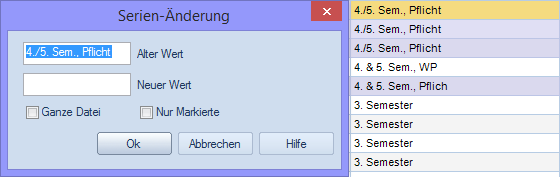
\includegraphics[width=1\textwidth]{serien-anderung}
	\vspace{-15pt}
	\caption{Serien Änderung}
	\label{fig:serien-anderung}
\end{figure}

\noindent
Im \figref{fig:serien-anderung} habe ich vier Felder markiert. Ich kann nach dieser Markierung direkt einen neuen Wert eintragen, die in allen markierten Felder übernommen wird. Darüber hinaus bietet mir die \texttt{Serien-Änderung} Schnittstelle viele weitere Möglichkeiten. In der Ansicht reicht es vollkommen aus, nur einen Feld auszuwählen, denn standardmäßig werden alle angezeigte Werte der Spalte miteinbezogen. Man kann diese ausdehnen, indem man ein Häkchen bei \texttt{Ganze Datei} setzt, diese beeinflusst auch die durch Filterung ausgeblendeten Werte. Den Einflussbereich kann man auch durch Markieren und die Auswahl von \texttt{Nur Markierte} einschränken. Sofern ein Wert in \texttt{Alter Wert} eingetragen ist, werden nur die Einträge, in den dieser Wert vorkommt, durch den neuen Wert geändert. 

\subsubsection{Sortieren (manuell)}
{\small\textit{implizti verfügbar in Stammdaten- und Unterricht-Ansichten\\}\par}

\noindent
Zusätzlich zum automatischen sortieren gibt es zwei Arten von manuelle Sortierung. Erstens kann man einzelne Zeilen per Drag \& Drop in der gewünschten Reihenfolge anordnen. Die hierdurch erzeugte Sortierung wird dauerhaft gespeichert. Man kann auch die Spaltennamen anklicken, diese sortiert die Einträge entsprechend der Werte, die in dieser Spalte eingetragen sind. Weitere Klicks ändern die Sortierrichtung. Diese Methode sortiert die vorhandene Einträge nur vorübergehend.

\section{Allgemeine Datenpflege}

\subsection{Nicht Editierbare Felder}
\label{sec:nicht-editierbar}

Grundsätzlich gilt: alle Felder mit blauem oder grauem Hintergrund sind nicht editierbar. Diese Werte werden entweder von Untis selbst gefüllt oder vererbt.

\subsection{Werte Kopieren}
\label{sec:werte-kopierung}

Das Kopieren von Werten in der Version 2015 funktioniert nicht mehr. Es können nur noch ganze Datensätze kopiert werden.

\subsection{Felder mit mehrere Angaben}
\label{sec:mehrfache-angaben}

Es gibt Felder in Untis, die mit mehrere Ressourcen befüllt werden können. Um die Ressourcen auszuwählen, verwendet man die STRG Taste und klickt die gewünschte Werte an. Man kann auch die Namen, durch einem Komma getrennt, hintereinander schreiben. In 2014 gab es auch Autovervollständigungsvorschläge. Als man einen Vorschlag mit der Eingabe-Taste angenommen hat, wurde sie einfach übernommen. Der Fokus blieb im Feld um ggf. weitere Ressourcen, Komma-getrennt, hinzuzufügen. In der Version 2015 gibt es nicht mehr Autovervollständigung, sondern Auswahlmöglichkeiten werden direkt angezeigt. Sobald man sich für eine Möglichkeit mit der Eingabe-Taste entschieden hat, wird der Fokus das nächste Feld weiter gegeben.

\section{Formate}
\label{sec:formate-dialog}

Formate sind festgelegte Darstellungen von Ressourcen. Wegen der Zwiespalt in der Untis-Benutzer-führung, zwischen Stammdaten/Unterrichte und Stundenpläne, werden sowohl hier als auch in \secref{sec:formate}, behandelt. Die Beschreibungen hier betreffen Stammdaten- und Unterricht-Ansichten. Man kann zwischen Formate mittels die Auswahlbox im unteren rechen Bereich des Fensters wechseln.

\subsection{Formate Ändern}

Um Ihren Umgang mit Untis zu erleichtern werden Sie oft die dargestellte Informationen anpassen wollen. Es gibt viele Änderungen die man vornehmen kann. Bis jetzt würden zwei davon in \secref{sec:symbolleiste-aktionen}, erwähnt: das ein- oder ausblenden von Attribute über \nameref{sec:felder-der-ansicht} und Schriftanpassungen über  \nameref{sec:einstellungen}. Es gibt aber zwei weitere Anpassungen, die man vornehmen kann.\\
\\
Sollte man Spalten ein- oder ausgeblendet haben, wird nach der aktuell angezeigte Format ein ``*" \hspace{1pt} an den Namen angehängt, um Ihnen zu zeigen, dass Sie Änderungen vorgenommen haben. Bei andere Änderungsarten wird jedoch kein ``*" \hspace{1pt} angehängt.

\subsubsection{Spaltenreihenfolge Ändern}

Ähnlich wie die manuelle Sortierung, kann man die Reihenfolge von Attribute-Spalten festlegen, indem man sie anklickt und an der gewünschte Position zieht.

\subsubsection{Spaltenbreite}
Wenn man die Trennung zwischen zwei Spalten bewegt ändert sich die Breite der erste der beiden Spalten entsprechend.

\newpage

\subsection{Formate speichern}

\begin{wrapfigure}{r}{.4\textwidth}
	\vspace{-14pt}
	\centering
	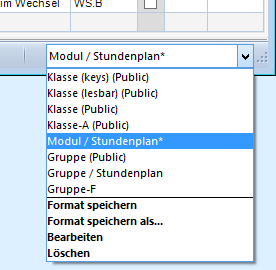
\includegraphics[width=.38\textwidth]{format-speichern}
	\vspace{-5pt}
	\caption{Formatbox}
	\label{fig:format-speichern}
	\vspace{-35pt}
\end{wrapfigure}

Um die vorgenommene Änderungen wieder aufrufbar zu machen, speichert man die als \texttt{Formate}. Dies wird vorgenommen durch die zuvor erwähnte Auswahlbox in der unteren rechten Ecke des Fensters.

\subsubsection{Format Speichern}

Speichert alle vorgenommene Änderungen zur aktuellen Ansicht in der aktuelle Ansicht. Sollte man eine Ansicht, die nicht von einem Benutzer erstellt wurde, geändert haben, wird doch eine neue Ansicht angelegt. Dieses Verhalten wird aber erst bemerkbar wenn ein andere Benutzer die 'selbe' Ansicht verwendet und sie sieht komplett anders aus.

\subsubsection{Format speichern als...}

\begin{wrapfigure}{r}{.4\textwidth}
	\vspace{-14pt}
	\centering
	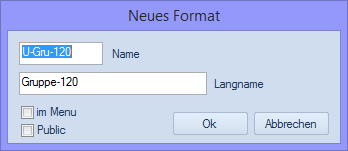
\includegraphics[width=.38\textwidth]{neues-format}
	\vspace{-5pt}
	\caption{Neues Format}
	\label{fig:neues-format}
	\vspace{-15pt}
\end{wrapfigure}

Speichert die vorgenommene Änderungen als ein neues Format. Nach der Auswahl wird ein Dialog geöffnet in dem man einen neuen Namen und Langnamen angeben kann. Hier kann man auch ein Häkchen setzten, um die Ansicht dem respektiven Stammdatenmenü hinzuzufügen, oder das Format alle Benutzer der Schule zugänglich zu machen. Sollte mehrere Benutzer häufig auf die selben Daten zugreifen ist es auf jeden Fall empfehlenswert diese zwei Häkchen zu setzen.

\subsubsection{Bearbeiten}

Öffnet die gleiche Dialog wie bei \texttt{Format speichern als...} mit einer anderen Beschriftung. Hier kann man vorhandene Formate umbenennen, sowie nachträglich die Häkchen für den Menüeintrag und Veröffentlichung setzen oder entfernen.

\subsubsection{Löschen}

Löscht die aktuelle Ansicht. Sollte dieses Format nicht von einem Benutzer erstellt sein, kann es unter Umständen dazu führen, dass das Programm abstürzt.
 
